The bar chart below shows the evolution of the number of commits and authors in Git through time, grouped by quarters.

\begin{tabular}{p{9cm} p{5cm}}
	\vspace{0pt} 
	\hspace*{-6cm}  
	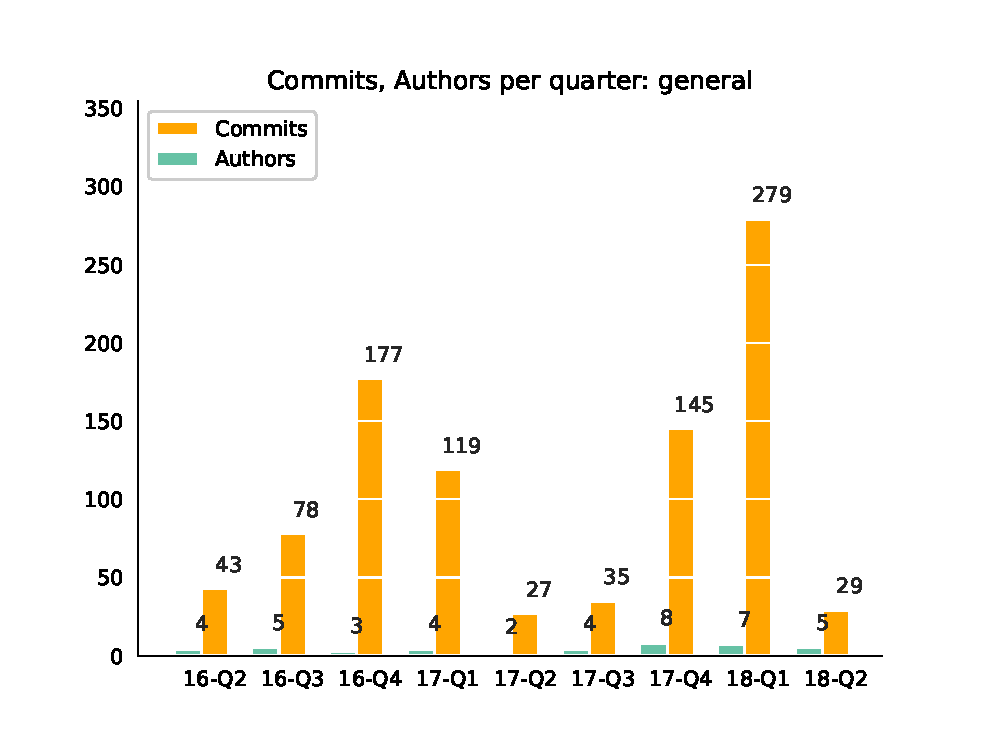
\includegraphics[scale=.75]{activity/git_commits_git_authors.eps}
	& 
	\vspace{0pt}
	\begin{tabular}{l|r|r|}
		% specify table head
		\bfseries Period & \bfseries Commits & \bfseries Authors
		% use head of csv as column names
		\csvreader[head to column names]{activity/git_commits_git_authors.csv}{}
		{\\\Date & \commits & \authors}
	\end{tabular}
\end{tabular}

%The total number of contributors divided into three sets (core,
%regular and casual\footnote{Contributing developers are characterized
%as core, regular and casual depending on their activity in the git
%repositories. The classification is built by sorting contributors by
%their total number of commits; we sum the total commits per each
%individual contributors: the individuals whose commits sum up to 80\%
%of the total number of commits in the quarter are the core
%contributors in that quarter. The regular contributors are those whose
%commits sum up to 95\% of the total. The others are the casual
%contributors.}) follow a similar pattern.

%\begin{figure}[H]
%    \centering
%    \includegraphics[scale=.35]{figs/onion.eps}
%    \caption{Evolution during the last quarters of core, regular and casual developers (based on git activity)}
%\end{figure}

%\begin{table}[H]
%    \centering
%    \begin{tabular}{l|r|r|r|}%
%    \bfseries Period & \bfseries Core & \bfseries Regular & \bfseries Occasional% specify table head
%    \csvreader[head to column names]{data/onion_model.csv}{}% use head of csv as column names
%    {\\\labels & \core & \regular & \occasional}
%    \end{tabular}
%    \caption{Characterization of developers by their total contribution to the project}
%\end{table}
